\chapter*{Задание 1}

Практикум 2 выполнялся по варианту 4.

\textbf{Задание}: Выполнить визуализацию неориентированного графа, представленного в формате tsv. 
Каждая строчка файла представляет собой описание ребра, сотоящее из трех чисел (Вершина,Вершина,Вес) или двух чисел (Вершина,Вершина). 
Во втором случае вес ребра принимается равным 1.

Для выполнения данного задания были изменены файлы с кодом примера.

В листинге \ref{listing_create} представлено создание и передача данных из буфера.

\begin{center}
	\begin{lstlisting}[label=listing_create,caption=Создание и передача данных из буфера]
unsigned int* host2gpc_ext_buffer[LNH_GROUPS_COUNT][LNH_MAX_CORES_IN_GROUP];
unsigned int edge_count = get_edge_count(SRC_FILE);
unsigned int messages_count = 0;
unsigned int u, v, w;

__foreach_core(group, core)
{
	host2gpc_ext_buffer[group][core] = (unsigned int*)lnh_inst.gpc[group][core]->external_memory_create_buffer(2 * 3 * sizeof(int) * edge_count); //2*3*sizeof(int)*edge_count);
	
	std::ifstream fin(SRC_FILE);
	for (int edge = 0; edge < edge_count; ++edge) 
	{
		fin >> u >> v >> w;
		EDGE(u, v, w);
		EDGE(v, u, w);
		messages_count += 2;
	}
	fin.close();
	
	
	lnh_inst.gpc[group][core]->external_memory_sync_to_device(0, 3 * sizeof(unsigned int)*messages_count);
}
	\end{lstlisting}
\end{center}

Для получения количества рёбер используется функция \textit{get\_edge\_count}, код которой представлен в листинге \ref{listing_count}.

\begin{center}
	\begin{lstlisting}[label=listing_count,caption=Создание и передача данных из буфера]
int get_edge_count(std::string filename)
{
	std::ifstream fin(filename);
	printf("%d\n", fin.is_open());
	int a1, a2, a3;
	int count = 0;
	while (fin >> a1 >> a2 >> a3)
	++count;
	fin.close();
	return count;
}		
	\end{lstlisting}
\end{center}

После заполнения графа данными, с помощью сервера boken визуализируется граф (рис. \ref{graph}).

\begin{figure}[ht!]\centering
	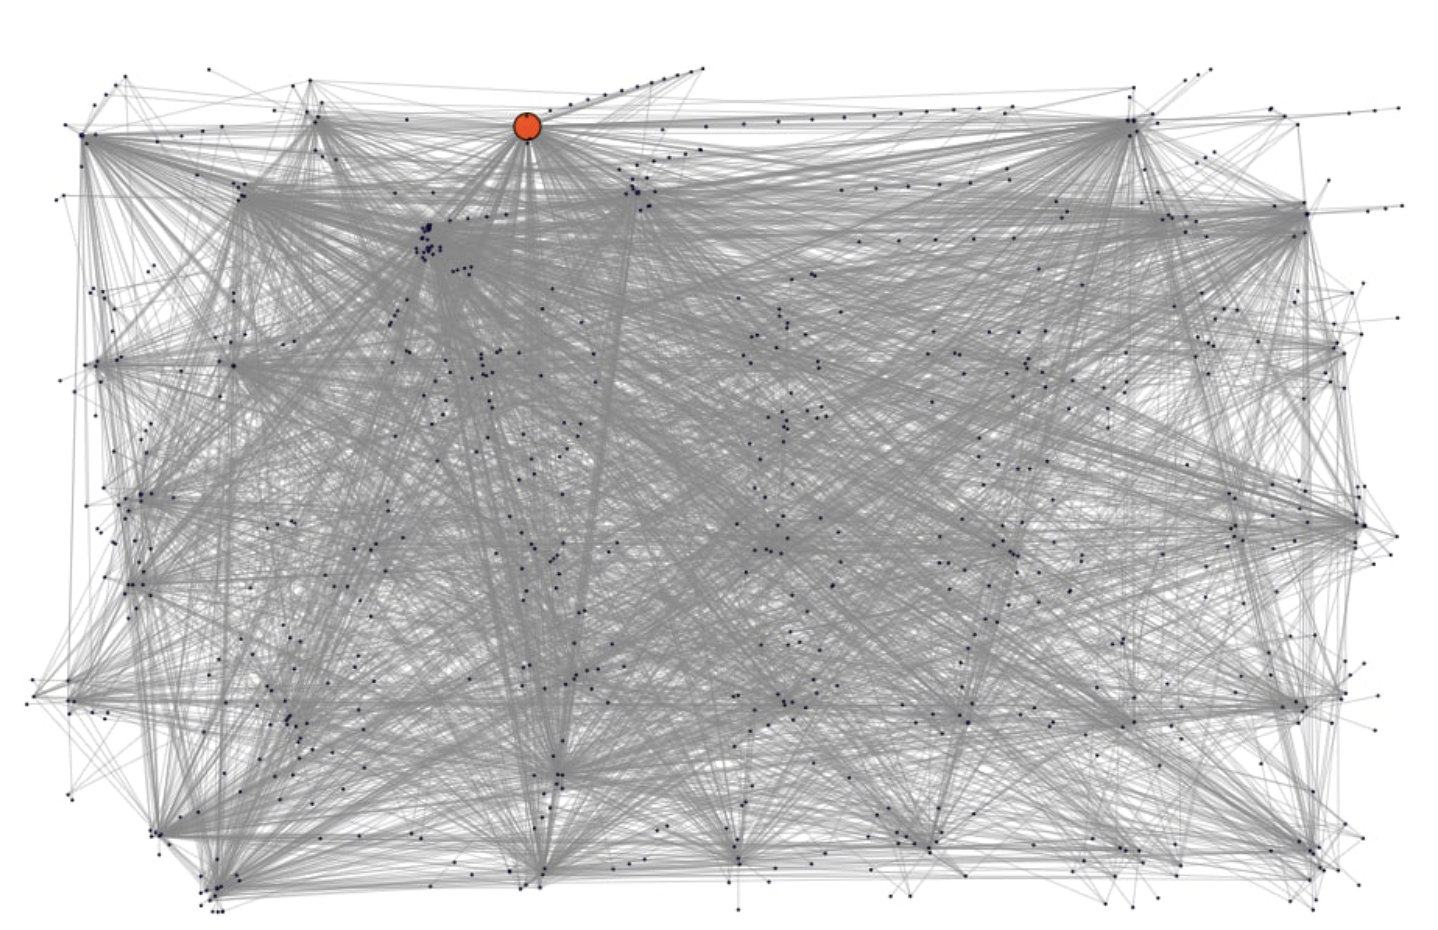
\includegraphics[scale=0.7]{graph}
	\caption{Визуализированный граф по варианту}
	\label{graph}
\end{figure}
